\section{Evaluation}
We compare the performance of this system with that of BPFS and ext4 file systems to evaluate its design and implementation. We use the performance of BPFS as a baseline and focus on following key questions:
\begin{itemize}
\item What is the cost and overhead of the anti caching mechanism on top of the BPFS system?
\item How does the degree of hotness and coldness of stored data affect the performance of the system?
\item How does this file system perform for different cache eviction threshold? (Improve this)
\end{itemize}

\subsection{Method}
Making a meaningful performance comparison of this system with both the memory based file system such as BPFS and the disk based file system such as ext4 presents presents challenges at different levels. We cannot make comparison in isolation since our implementation is a hybrid approach that incorporates both systems. Another difficulty is that for a disk based file systems, such as ext4 that runs in the kernel layer, several parameters and behaviors are opaque to users and we have very limited contol on enforcing the pure disk-based behaviors. For instance, ext4 filesystems performs several operations in memory and commit to the disk only periodically [cite{something}]. 

For the purpose of the evaluation, we run our experiments on a real hardware with 8 CPU cores running RedHat Linux Operating Systems with 16 GM of memory, 500 GB of Solid state Drive and * MB cacheline. We simulate the behavior of NVM on the DRAM due to unavailability of the hardware (really???). Unless otherwise noted, both the original and our implementation of BPFS are mounted in the memory with 2 GB image. The anticaching daemon is set to run at 10 ms by default with caching occupancy threshold of 40 MB. These values were chosen by performing emperical analysis.    

\subsection{Experimental evaluations}
In this section we present the experimental evaluations of this file system using differnt micro and macro benchmarks and throughput evalations and offer comparisons with those of BPFS and ext4 file-systems. 


\subsubsection{Microbenchmark: Various File Operations}
In order to ensure the correctness of various file operations and to measure cost of additional overheads due to added behaviors such as anti-caching, we benchmarked 40 different file operations. We used 'timeit' package in Python programming language to measure the time for these operations. Table 5.1 shows a representative sample of those operations for both AC\-BPFS and BPFS. The table shows that for the file operations the added overhead is negligible, if any at all. We also performed similar benchmarks for all the file operations in the ext4 file system. Since the time taken for each of the file operations were in the order of one tenth of a millisecond without fsync and in the order of 10 milliseconds with fync enabled, the benchmarks for the operations in the ext4 file systems are not shown in the table.

\begin{table}[!t]
%\vspace{0.1in}
\begin{center}
{\footnotesize
\begin{tabular}{c|c|l}
\textbf{Operations} & \textbf{Anti Cache BPFS(ms)} & \textbf{BPFS(ms)} \\
\hline
chmod&5.26&5.19 \\
create&6.49&6.45 \\
link&6.21&6.24 \\
mkdir&6.61&6.55 \\
read&4.67&4.61 \\
readdir&3.24&3.1 \\
rename\_dir\_intra&8.3&7.61 \\
rename\_file\_inter&8.6&7.82 \\
rmdir&6.66&5.95 \\
symlink&6.58&6.46 \\
unlink\_16M&10.03&10.42 \\
unlink\_hardlink&5.5&5.5 \\
write\_1M\_4k&6.91&6.22 \\

\end{tabular}
}
\end{center}
\vspace{-0.1in}
\mycaption{tbl-micro}{Microbenchmark}{\footnotesize The table
shows XXXX
}
\end{table}

 \begin{figure*}[t]\centering
\begin{subfigure}{.46\textwidth}
  \centering
  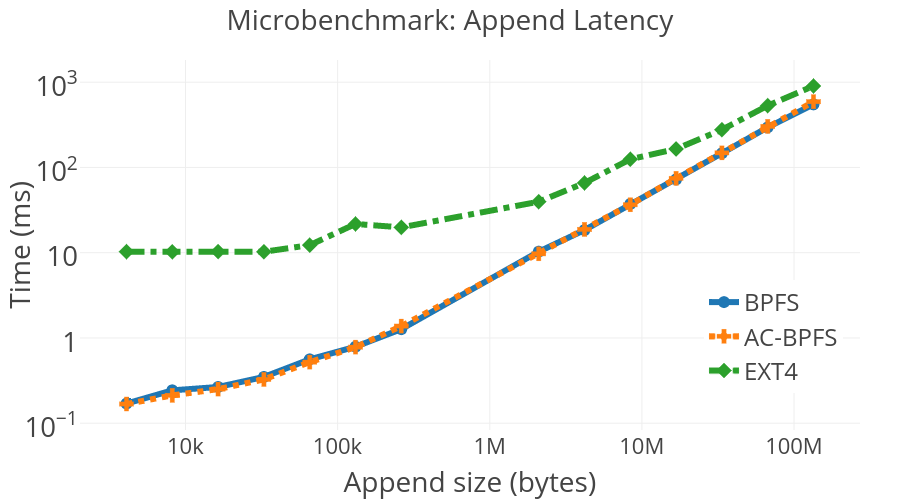
\includegraphics[width=\linewidth]{figs/append.png}
 \mycaption{fig-append}{Design Overview of BPFS}{\footnotesize The figure shows the overall design of our system. XXX}
\end{subfigure}
\begin{subfigure}{.46\textwidth}
  \centering
  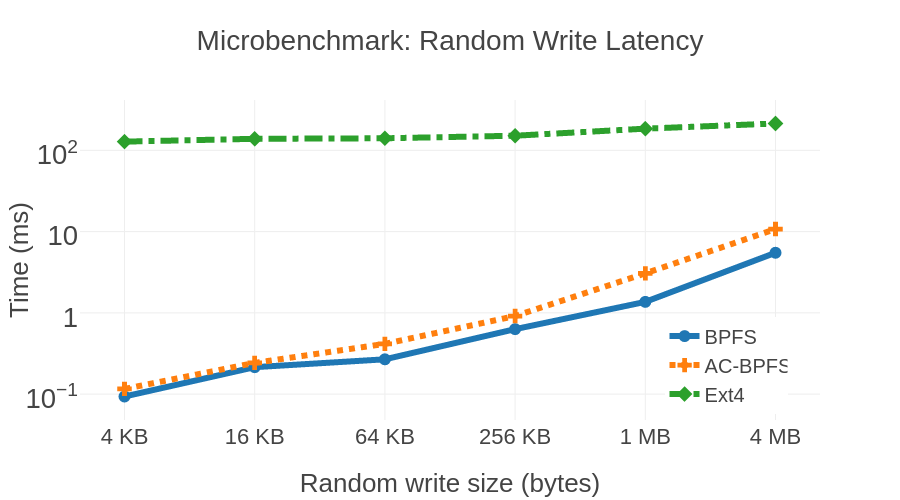
\includegraphics[width=\textwidth]{figs/write.png}
\vspace{-0.2in}
\mycaption{fig-write}{Design Overview of BPFS}{\footnotesize The figure shows the overall design of our system. XXX}
\end{subfigure}
\caption{Microbenchmarks}
\label{fig:fig}
\end{figure*}

\subsubsection{Microbenchmark: Random write}
. We evaluated the performance of making random write operations for various data size for AC\_BPFS, BPFS and ext4. For the AC\-BPFS, to ensure uniform distribution of write operations to data blocks in both the persistent memory and the disk, we pre-generated a list of files of various sizes and random offsets with in those files. We ensured that data chucks written at random offsets exceeded the pre-specified cache threshold to force seek from the disk. We called 'fsync' after every write call to force the data to disk so as to make even comparisons across the filesystems. We used UNIX 'clock\_gettime' system call to measure the time for this benchmark.

Figure~\ref{fig-write} shows the results for this micro-benchmark. Both AC\_BPFS and BPFS are faster than the ext4 in orders of magnitude, as we hoped. It also shows that AC\-BFPS, although starts to lag behind the BPFS as the size of the data being written increases, it does not lag significantly, that reinforces our initial intuition and supports our objective.



\subsubsection{Microbenchmark: Append}
We measured the cost of appending data chunks of various size to an empty file. As with the benchmark for the random write, we called ‘fsync’ after every write call to ensure that the data gets written to the disk. We used UNIX 'clock\_gettime' system call to measure the time for this benchmark.

As with random write, Figure 5.1(b) shows that both AC\-BPFS and BPFS are faster than the ext4 in orders of magnitude. Since the writing of all the data for the ‘append’ operation happened entirely in memory, AC\-BPFS and BPFS performance lines are virtually inseparable. This result justifies the anti-caching mechanism that we have employed and also illustrates its low overhead.


\subsubsection{Microbenchmark: Degree of coldness}
This synthetic benchmark is used to demonstrate the effect of storing hot data in NVM and cold data on disk. The experimental setup consists of a 2GB NVM, a 400MB eviction threshold. Initially a 1GB file is written to both the file system, which triggers the anti-cache manager to evict 600MB of the file onto the disk and the remaining 400MB remains in the NVM. For varying degrees of coldness (say X), reads are performed to various blocks of the file either located on disk or NVM to ensure that X\% of the block reads are from disk and the remaining block reads are from NVM. So as the graph indicates, when the degree of coldness is 100\%, it implies that all the reads performed by the workload are from disk and the read latency is similar to that of ext4 as expected. But as the degree of hotness becomes 40\%, the read latency decreases in AC-BPFS as the number of disk reads decreases but this triggers eviction by the anti-cache manager. This introduces a slight additional overhead during each read because some of the blocks that were expected to be in the NVM could have gotten evicted and hence would result in a disk read. This graph also proves that the rate of decline in the read latency increases as as the degree of coldness decreases since the number of blocks evicted decreases and thus the probability of reading from NVM increases.


\begin{figure}
\centering
\vspace{-0.2in}
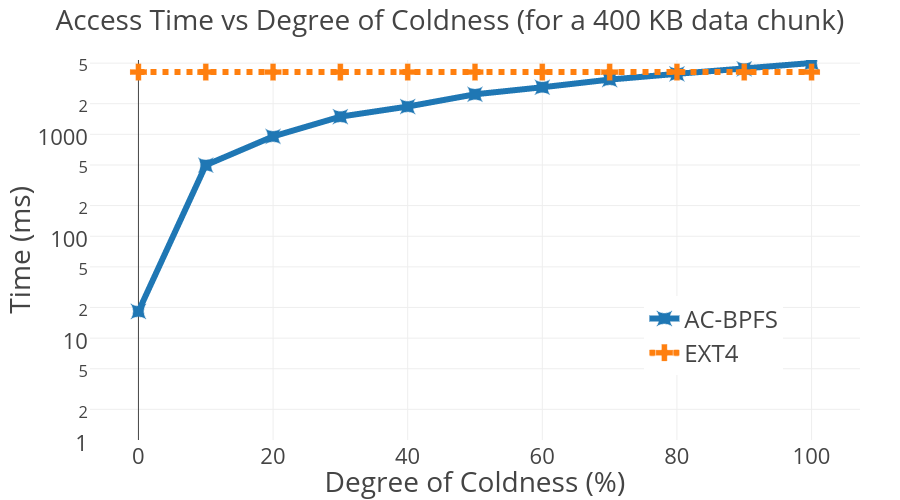
\includegraphics[width=0.5\textwidth]{figs/coldness.png}
\vspace{-0.2in}
\mycaption{fig-coldness}{BPFS tree}{\footnotesize The figure shows the overall design of our system. XXX}
\end{figure}

 
\subsubsection{Macrobenchmark: File Bench}
 For this benchmark, we used FileBench to test and compare the performance of the three files systems by generating a large variety of workloads {cite} of size 1.25 GB. The workload is comprised of 33\% read requests and 67\% write requests. For the AC\-BPFS, we ran the benchmark by varying the (anti) caching thresholds – from 20\% of the workload size to 100\% of the workload size. We did so in order to get insights on the effectiveness and overheads of the anti-caching mechanisms in addition to making comparison of the AC\-BPFS with BPFS and ext4 file systems.


 \begin{figure*}[t]\centering
\begin{subfigure}{.46\textwidth}
  \centering
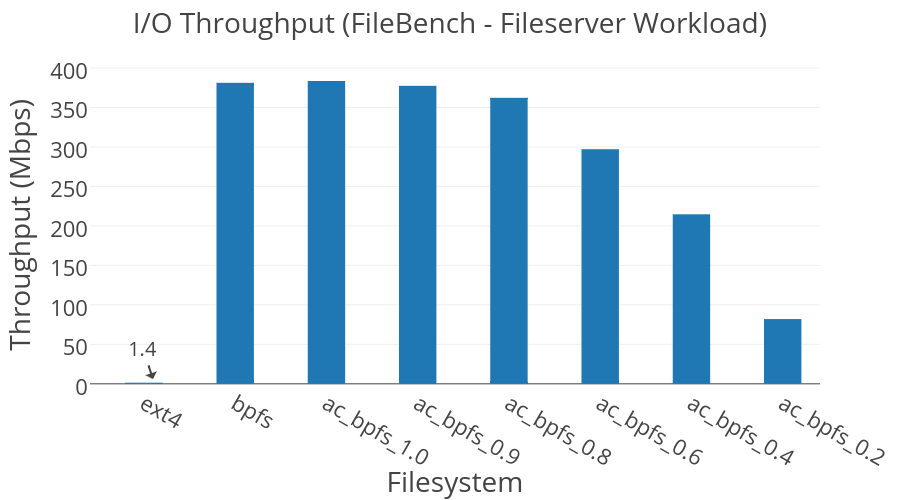
\includegraphics[width=\textwidth]{figs/filebench.png}
 \mycaption{fig-fb}{Design Overview of BPFS}{\footnotesize The figure shows the overall design of our system. XXX}
\end{subfigure}
\begin{subfigure}{.46\textwidth}
  \centering
  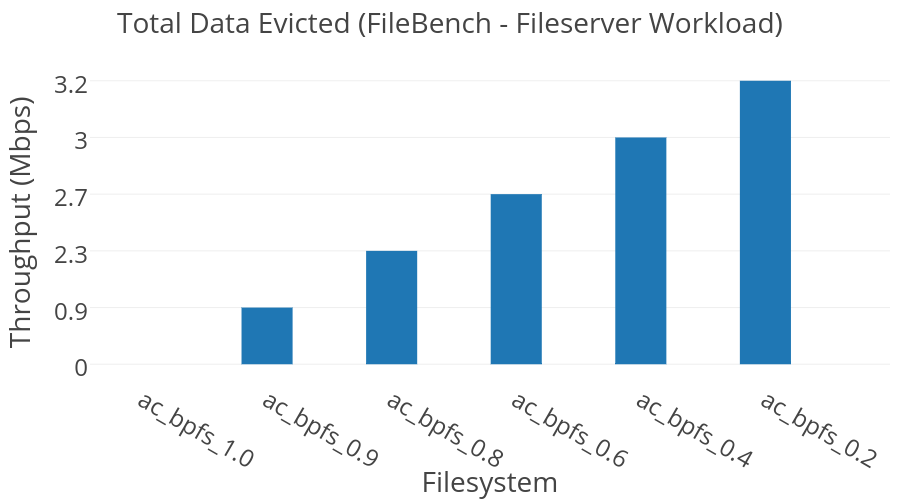
\includegraphics[width=\textwidth]{figs/bench2.png}
\vspace{-0.2in}
\mycaption{fig-fb2}{Design Overview of BPFS}{\footnotesize The figure shows the overall design of our system. XXX}
\end{subfigure}
\caption{Macrobenchmarks}
\label{fig1:fig1}
\end{figure*}

The figure shows that when the caching threshold is 100\% of the workload size (i.e. all the operations happen in the persistent memory), the performance of AC\-BPFS is identical to that of BPFS, as we expected. As we decrease the caching threshold, the performance suffers accordingly. On all times, the performance of the AC\-BPFS is better than that of ext4 in orders of magnitude.
